\section{单圆线解析与二维校准}
\label{chapter:03}

% block-id: 03.round_derivation.heading
\hypertarget{03.round_derivation.heading}{}
\subsection{圆线径向方程与归一化}

% block-id: 03.round_derivation.p1
\hypertarget{03.round_derivation.p1}{}
长直圆线内部的轴向电流满足 (1/r)d(r dJz/dr)/dr=κ²Jz。轴心有限性确定径向函数为 I\(_0\)(κr)，总复电流约束与积分关系 \(\int\)\(_0\)\(^a\)rI\(_0\)(κr)dr=aI\(_1\)(κa)/κ 确定其系数。表面轴向电场与总电流之比给出单位长度内部阻抗；对电流密度独立执行焦耳积分，可核对阻抗实部与损耗之间的关系。推导采用与正文一致的 RMS 相量。

% block-id: 03.analytic.heading
\hypertarget{03.analytic.heading}{}
\subsection{单圆线内部场校准}

% block-id: 03.analytic.p1
\hypertarget{03.analytic.p1}{}
长直圆线的径向电流与内部阻抗采用 \eqref{eq:E03}。200 kHz 下趋肤深度 δ=\metric{skin_depth} mm，约为圆线半径的 0.148，电流集中于表层。直流电阻为 \metric{q1_rdc} mΩ/m，交流电阻为 \metric{q1_rac} mΩ/m，Rac/Rdc=3.64720，对应损耗 \metric{q1_loss} W/m。径向曲线与截面幅值分别见 图~\ref{fig:q1_profile} 和 图~\ref{fig:q1_cross_section}。相位沿半径连续展开，显示了趋肤扩散同时引起的幅值衰减和相位变化；解析阻抗的范围为导体内部场。

% block-id: 03.analytic.p2
\hypertarget{03.analytic.p2}{}
独立二维圆盘扩散使用 353、1389、5573 节点的三档网格，并按总复电流归一化。随着网格细化，Rac 解析相对误差由 7.05×10⁻³ 降至 2.30×10⁻⁴，最终为 1.79×10⁻⁶；最细档功率积分相对差为 3.07×10⁻⁶，见 图~\ref{fig:q1_fem_error}。这组结果验证了孤立圆线内场问题的离散、归一化与功率后处理。截面图通过径向解析样本的线性插值和轴对称映射得到，后续多股模型则使用其实际导体场解。

% block-id: 03.equation.E03
\hypertarget{03.equation.E03}{}
\hypertarget{E03}{}
\begin{equation}
\begin{gathered}
\delta=(\pi f\mu\sigma)^{-1/2} \\
\kappa=(1+j)/\delta \\
J_z(r)=\frac{I_t\kappa I_0(\kappa r)}{2\pi a I_1(\kappa a)} \\
z_{\mathrm{int}}=\frac{\kappa I_0(\kappa a)}{2\pi a\sigma I_1(\kappa a)}
\end{gathered}
\tag{3}\label{eq:E03}
\end{equation}

% block-id: 03.figure.q1_profile
\hypertarget{03.figure.q1_profile}{}
\begin{figure}[!htbp]
\centering
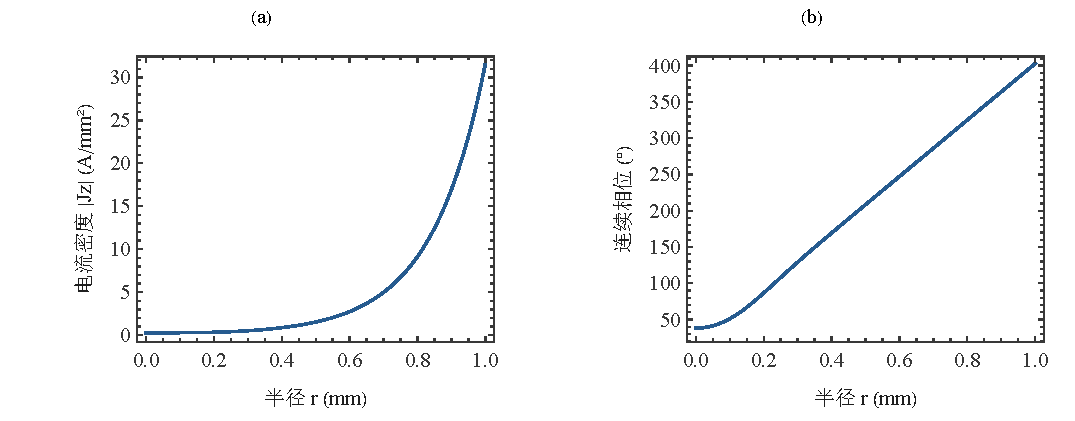
\includegraphics[width=\linewidth,height=.72\textheight,keepaspectratio]{../../assets/zh-CN/q1_profile.pdf}
\caption{单圆线径向电流幅值与相位。 铜导体直径 2 mm，200 kHz、20 A RMS。 (a) RMS 幅值；(b) 连续显示的相位。 相位显示采用径向连续提升，幅值保留 RMS 归一化。径向样本来自保存的 Bessel 解析数据。}
\label{fig:q1_profile}
\end{figure}

% block-id: 03.figure.q1_cross_section
\hypertarget{03.figure.q1_cross_section}{}
\begin{figure}[!htbp]
\centering
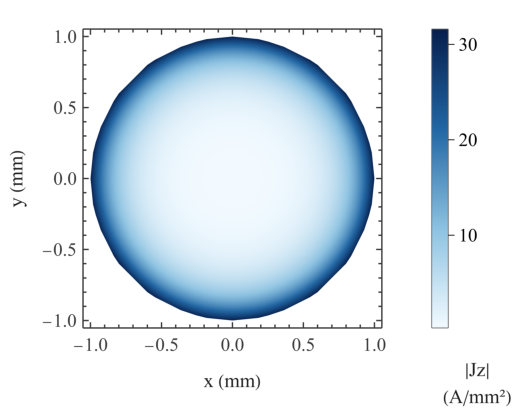
\includegraphics[width=\linewidth,height=.72\textheight,keepaspectratio]{../../assets/zh-CN/q1_cross_section.pdf}
\caption{单圆线解析截面幅值。 铜导体直径 2 mm，200 kHz、20 A RMS。 色标显示轴向 RMS 电流密度。 径向样本经线性插值后作轴对称映射。坐标以毫米显示，电流密度以 A/mm² 显示。}
\label{fig:q1_cross_section}
\end{figure}

% block-id: 03.figure.q1_fem_error
\hypertarget{03.figure.q1_fem_error}{}
\begin{figure}[!htbp]
\centering
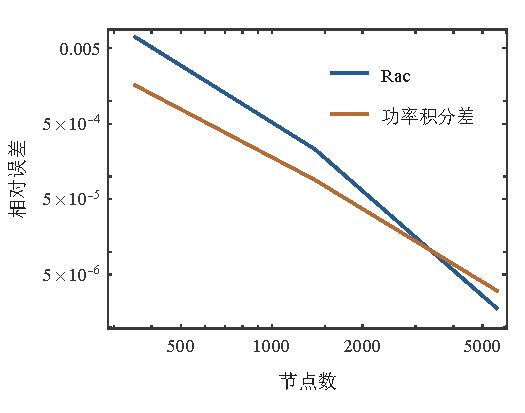
\includegraphics[width=\linewidth,height=.72\textheight,keepaspectratio]{../../assets/zh-CN/q1_fem_error.pdf}
\caption{单圆线二维校准误差。 铜导体直径 2 mm，200 kHz、20 A RMS。 三档网格与独立功率积分对应同一内场问题。 电阻参照为相同圆线的内部 Bessel 解。功率使用独立材料域积分计算。}
\label{fig:q1_fem_error}
\end{figure}
